\begin{activity} \label{A:3.1.1} A water tank has the shape of an inverted circular cone (point down) with a base of radius $6$ feet and a depth of $8$ feet.  Suppose that water is being pumped into the tank at a constant instantaneous rate of $4$ cubic feet per minute.
\ba
	\item Draw a picture of the conical tank, including a sketch of the water level at a point in time when the tank is not yet full.  Introduce variables that measure the radius of the water's surface and the water's depth in the tank, and label them on your figure.
	\item Say that $r$ is the radius and $h$ the depth of the water at a given time, $t$.  What equation relates the radius and height of the water, and why?
	\item Determine an equation that relates the volume of water in the tank at time $t$ to the depth $h$ of the water at that time.
	\item Through differentiation, find an equation that relates the instantaneous rate of change of water volume with respect to time to the instantaneous rate of change of water depth at time $t$.
	\item Find the instantaneous rate at which the water level is rising when the water in the tank is $3$ feet deep.
	\item When is the water rising most rapidly:  at $h = 3$, $h = 4$, or $h = 5$?
\ea
\end{activity}
\begin{smallhint}
\ba
	\item[(b)] Think about similar triangles.
	\item[(c)] Recall that the volume of a cone is $V = \frac{1}{3} \pi r^2 h$.
	\item[(d)] Remember to differentiate implicitly with respect to $t$.
	\item[(e)] Use $h = 3$ and the fact that the value of $\frac{dV}{dt}$ is given.
	\item[(f)] Consider \href{http://gvsu.edu/s/9p}{\texttt{http://gvsu.edu/s/9p}}.  Why does this phenomenon occur?
\ea
\end{smallhint}
\begin{bighint}
\ba
	\item[(b)] Think about similar triangles and how the ratio of $r$ to $h$ must be constant.
	\item[(c)] Recall that the volume of a cone is $V = \frac{1}{3} \pi r^2 h$, and use the relationship established in (b) to write $r$ in terms of $h$.
	\item[(d)] Remember to differentiate implicitly with respect to $t$ and use the chain rule appropriately.
	\item[(e)] Use $h = 3$ and the fact that the value of $\frac{dV}{dt}$ is given.  Solve for $\frac{dh}{dt}$.
	\item[(f)] Consider \href{http://gvsu.edu/s/9p}{\texttt{http://gvsu.edu/s/9p}}.  Why does this phenomenon occur?
\ea
\end{bighint}
\begin{activitySolution}
\ba
	\item Letting $r$ represent the water's radius at time $t$ and $h$ the water's depth, we see the following situation:
	\begin{center}
	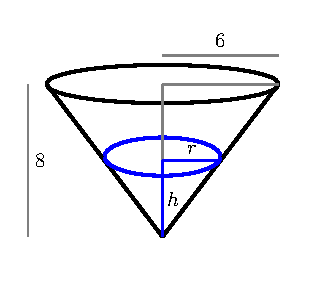
\includegraphics{figures/3_5_Act1Soln.eps}
	\end{center}
	\item Observe that the right triangle with legs of length $h$ and $r$ is similar to the right triangle with legs of length $8$ and $6$, respectively, based on how the water assumes the shape of the tank, and thus $\frac{r}{h} = \frac{6}{8}$, so that $r = \frac{3}{4}h$.
	\item Since the water in the tank always takes the shape of a circular cone, the volume of water in the tank at time $t$ is given by $V = \frac{1}{3}\pi r^2 h$.  Because we have established that $r = \frac{3}{4}h$, it follows that
	$$V = \frac{1}{3}\pi \left( \frac{3}{4}h \right)^2 h = \frac{3}{16} \pi h^3.$$ 
	\item Differentiating with respect to $t$, we now find
	$$\frac{dV}{dt} = \frac{1}{16} \pi h^2 \frac{dh}{dt},$$
	which relates the rates of change of $V$ and $h$.
	\item It is given in the problem setting that water is entering the tank at a rate of 4 cubic feet per minute, hence $\frac{dV}{dt} = 4$, and we are interested in the rate of change of the water's depth when $h = 3$.  Substituting these values into the equation that relates $\frac{dV}{dt}$ and $\frac{dh}{dt}$, we find that
	$$4 =  \frac{1}{16} \pi 3^2 \left. \frac{dh}{dt} \right|_{h=3},$$
	so that $\left. \frac{dh}{dt} \right|_{h=3} = \frac{64}{9\pi} \approx 2.2635$ feet per minute.
\ea
\end{activitySolution}
\aftera